\documentclass{article}
    \usepackage[utf8]{inputenc}
    \usepackage[spanish]{babel}
    \decimalpoint
    \usepackage{amsmath, amssymb, amsfonts}
    \usepackage{xparse, physics}
    \usepackage{cancel}
    \usepackage{graphicx}
    \usepackage[usenames]{color}
    \parindent  = 0mm
    \parskip    = 4mm
    \usepackage[text={20cm,25cm},centering,top=1.5cm,bottom=1.5cm,letterpaper,showframe=false]{geometry}

    \definecolor{azul}{RGB}{10,80,190}
    \definecolor{negro}{RGB}{0,0,0}
    \definecolor{rojo}{RGB}{190,80,10}
    \definecolor{verde}{RGB}{0,120,50}
    \renewcommand{\baselinestretch}{1.2}

    \begin{document}
        \title{Tarea/Examen 4 - Aplicaciones}
        \author{Careaga Carrillo Juan Manuel
        \\ Quiróz Castañeda Edgar
        \\ Soto Corderi Sandra del Mar}
        \date{Miércoles 1 de junio de 2018}
        \maketitle

        \begin{enumerate}
            % Ejercicio 1
            \item {
                Encontrar puntos máximos, mínimos y sillas de $f(x,y)=(x^2+y^2)e^{(y^2-x^2)}$.
                Graficar la función.

                \color{azul}
            }
            % Ejercicio 2
            \item {
                Encontrar máximos y mínimos de $f(x,y,z)=x^2y^2z^2$ con la restricción
                $x^2+y^2+z^2=1$.

                \color{azul}
            }
            % Ejercicio 3
            \item {
                Encontrar los valores máximos y mínimos absolutos para $f(x,y)=xy^2$ sobre
                la región $D=\{(x,y)|x\geq 0, y\geq 0 \text{ y } x^2+y^2\leq 3\}$.

                \color{azul}
            }
            % Ejercicio 4
            \item {
                Encontrar los puntos sobre el cono $z^2=x^2+y^2$ más cercanos al punto
                $(4,2,0)$.

                \color{azul}
            }
            % Ejercicio 5
            \item {
                Encontrar tres números positivos que sumen $12$ y cuya suma de sus cuadrados
                sea lo más pequeña posible.

                \color{azul}
            }
            % Ejercicio 6
            \item {
                Tres alelos, $A$, $B$ y $O$ determinan los 4 tipos de sangre, a saber
                $A(AA \text{ o } AO)$, $B(BB \text{ o } BO)$, $O(OO)$ y $AB$. La ley
                de Hardy-Weinberg establece que la proporción de individuos de una
                población que llevan dos alelos diferentes es
                \[ P=2pq+2pr+2rq \]
                donde $p$, $q$ y $r$ son las proporciones de $A$, $B$ y $O$ respectivamente
                en la población. Usar el hecho de que $p+q+r=1$ para demostrar que $P$
                es cuando mucho $\frac{2}{3}$.

                \color{azul}
                Del hecho $p+q+r=1$ tenemos que $p=1-q-r$, entonces la ecuación de
                Hardy-Weinberg queda
                \begin{eqnarray*}
                    P(p,q,r) & = & 2pq+2pr+2rq\\
                    P(q,r)   & = & 2(1-q-r)q+2(1-q-r)r+2rq\\
                             & = & 2q-2q^2-2rq+2r-\cancel{2rq}-2r^2+\cancel{2rq}\\
                             & = & -2\left(r^2+rq-r-q+q^2\right)
                \end{eqnarray*}
                De ésta última ecuación, obtendremos máximos y mínimos. Las primeras derivada
                parciales son:
                \begin{eqnarray*}
                    P_q(q,r)=-2\left(2q+r-1\right) &
                    P_r(q,r)=-2\left(2r+q-1\right)
                \end{eqnarray*}
                Por consiguiente $P_q(q,r)=0$ y $P_r(q,r)=0$ implican que
                \begin{eqnarray}
                    2q+r-1 & = & 0\\
                    2r+q-1 & = & 0
                \end{eqnarray}
                De {\bf\color{rojo} (1)} $r=1-2q$, sustituyendo en {\bf\color{rojo} (2)} $2(1-2q)+q-1=0 \Rightarrow 2-4q+q-1=0
                \Rightarrow q=\frac{1}{3} \therefore r=1-\frac{2}{3}=\frac{1}{3}$. Por lo
                que se deduce que existe un punto crítico en $(\frac{1}{3},\frac{1}{3})$.

                Para mostrar que dicho punto crítico es un máximo, encontremos sus segundas
                derivadas parciales:\\$P_{qq}(q,r)=-4;P_{rr}(q,r)=-4;P_{qr}(q,r)=-2$.

                Por la prueba de las segundas derivadas parciales, tenemos
                $P_{qq}P_{rr}-[P_{qr}]^2=(-4)(-4)-(-2)^2=16-4=12>0$ y puesto que $P_{qq}=-4<0$,
                entonces el punto $(\frac{1}{3},\frac{1}{3})$ es un máximo relativo. Más aún,
                como la función $P(q,r)$ representa un paraboloide, el punto $(\frac{1}{3},
                \frac{1}{3})$ es un {\bf máximo absoluto}.

                El valor máximo que alcanza la función es $P(\frac{1}{3},\frac{1}{3})=
                -2(\frac{1}{9}+\frac{1}{9}-\frac{1}{3}-\frac{1}{3}+\frac{1}{9})=
                -2(\cancel{\frac{3}{9}}-\cancel{\frac{1}{3}}-\frac{1}{3})=
                -2(-\frac{1}{3})=\frac{2}{3}$

                Por lo tanto el valor de la función $P$ es a lo más $\frac{2}{3}$
            }
            % Ejercicio 7
            \item {
                Reducir las ecuaciones a la forma canónica, clasificarlas, analizarlas
                usando trazas y otros planos, y bosquejar las gráficas:
                \begin{enumerate}
                    % a)
                    \item{
                        $x^2+2y-2z^2=0$
                        
                        \color{azul}
                        Despejando $y$, tenemos $\displaystyle y=z^2-\frac{x^2}{2}$
                        
                        Traza en el plano $XY$: $z=0 \Rightarrow y=-\frac{1}{2}x^2$
                        \begin{center}
                            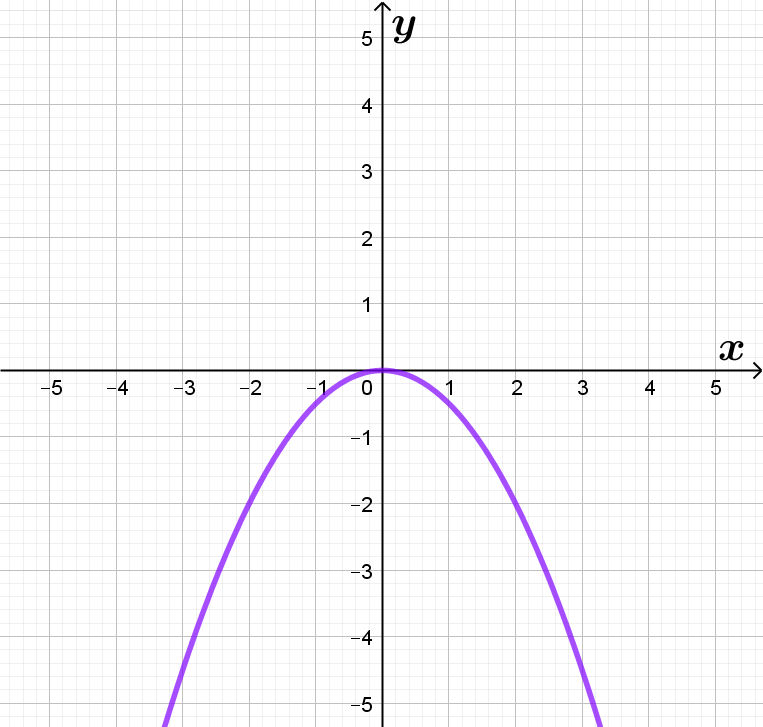
\includegraphics[width=4.5cm]{img/7a1.png}
                        \end{center}
                        Traza en el plano $XZ$: $y=0 \Rightarrow z^2-\frac{x^2}{2}=0$
                        \begin{center}
                            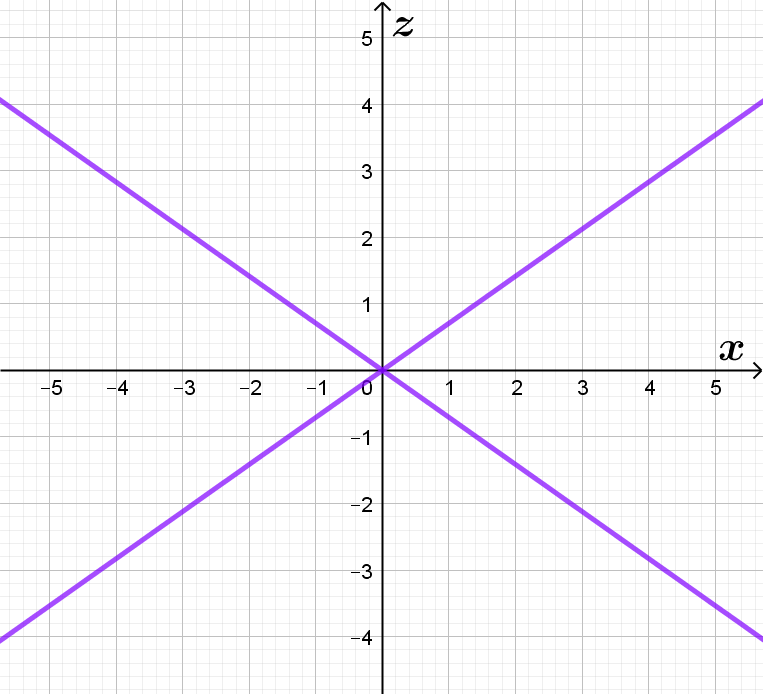
\includegraphics[width=4.5cm]{img/7a2.png}
                        \end{center}
                        Traza en el plano $YZ$: $x=0 \Rightarrow y=z^2$
                        \begin{center}
                            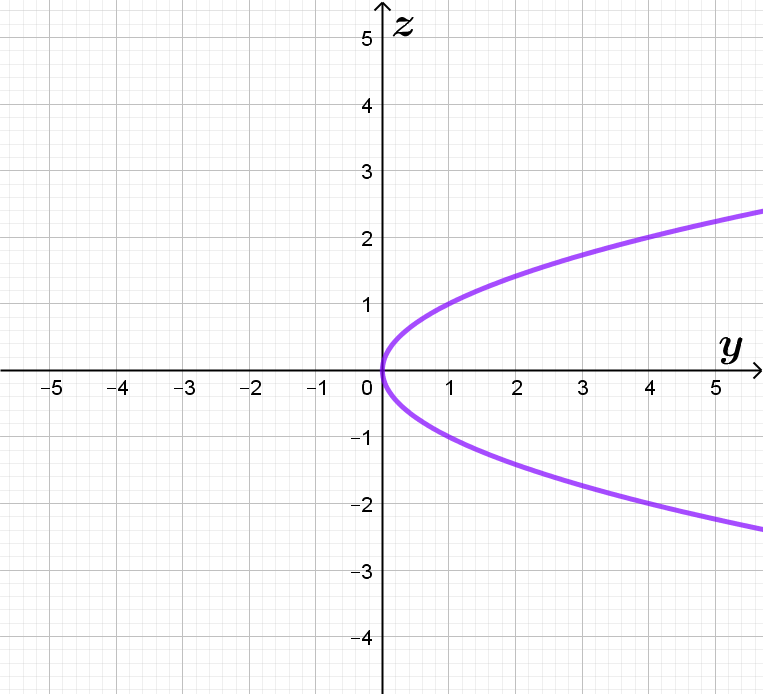
\includegraphics[width=4.5cm]{img/7a3.png}
                        \end{center}
                        La ecuación representa un {\bf paraboloide hiperbólico}
                        \begin{center}
                            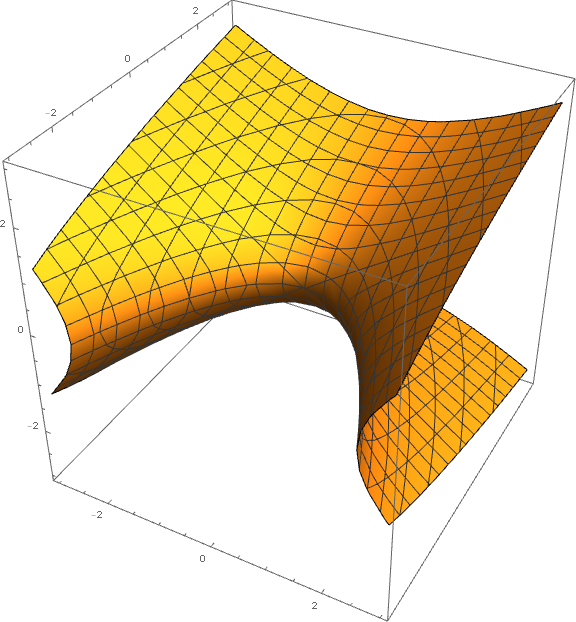
\includegraphics[width=6cm]{img/7a.png}
                        \end{center}
                    }
                    % b)
                    \color{negro}
                    \item{
                        $x^2-y^2+z^2-2x+2y+4z+2=0$
                        \color{azul}
                        \begin{eqnarray*}
                            (x^2-2x+1)-(y^2-2y+1)+(z^2+4z+4) & = & -2+4\\
                            (x-1)^2-(y-1)^2+(z+2)^2          & = & 2\\[.3cm]
                            \frac{(x-1)^2}{2}-\frac{(y-1)^2}{2}+\frac{(z+2)^2}{2}
                            & = & 1
                        \end{eqnarray*}
                        
                        En el plano $XY$:
                        \(
                            z=0 \Rightarrow
                            \frac{(x-1)^2}{2}-\frac{(y-1)^2}{2}+2=1\Rightarrow
                            \frac{(y-1)^2}{2}-\frac{(x-1)^2}{2}=1
                        \)
                        \begin{center}
                            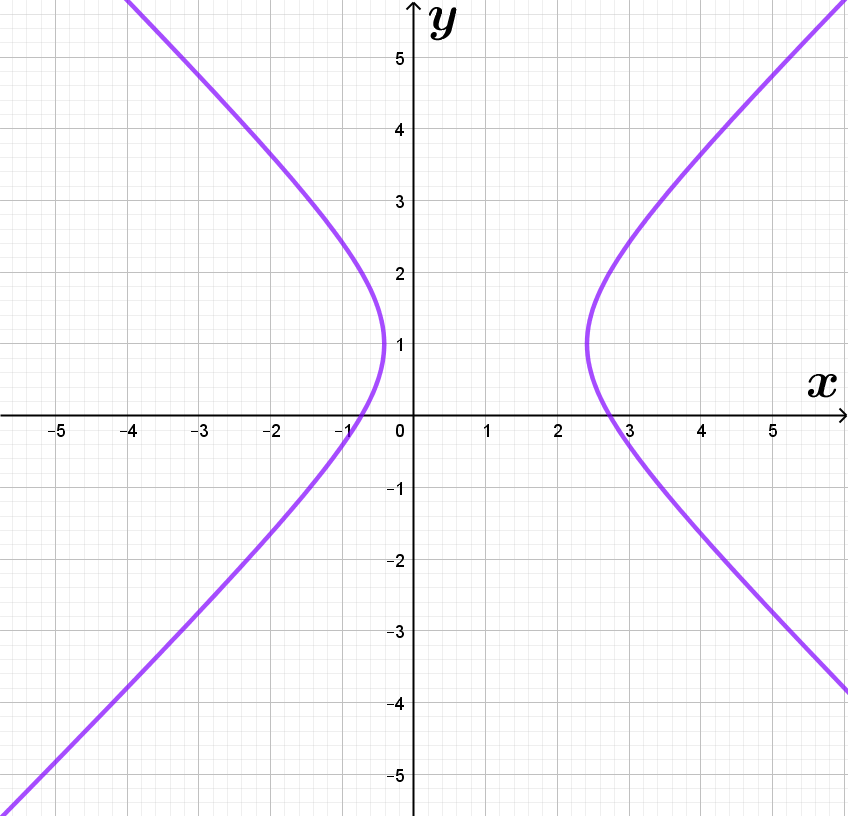
\includegraphics[width=4.5cm]{img/7b1.png}
                        \end{center}
                        En el plano $XZ$:
                        \(
                            y=0\Rightarrow
                            \frac{(x-1)^2}{2}-\frac{1}{2}+\frac{(z+2)^2}{2}=1\Rightarrow
                            \frac{(x-1)^2}{2}+\frac{(z+2)^2}{2}=\frac{3}{2}\Rightarrow
                            (x-1)^2+(z+2)^2=3
                        \)
                        \begin{center}
                            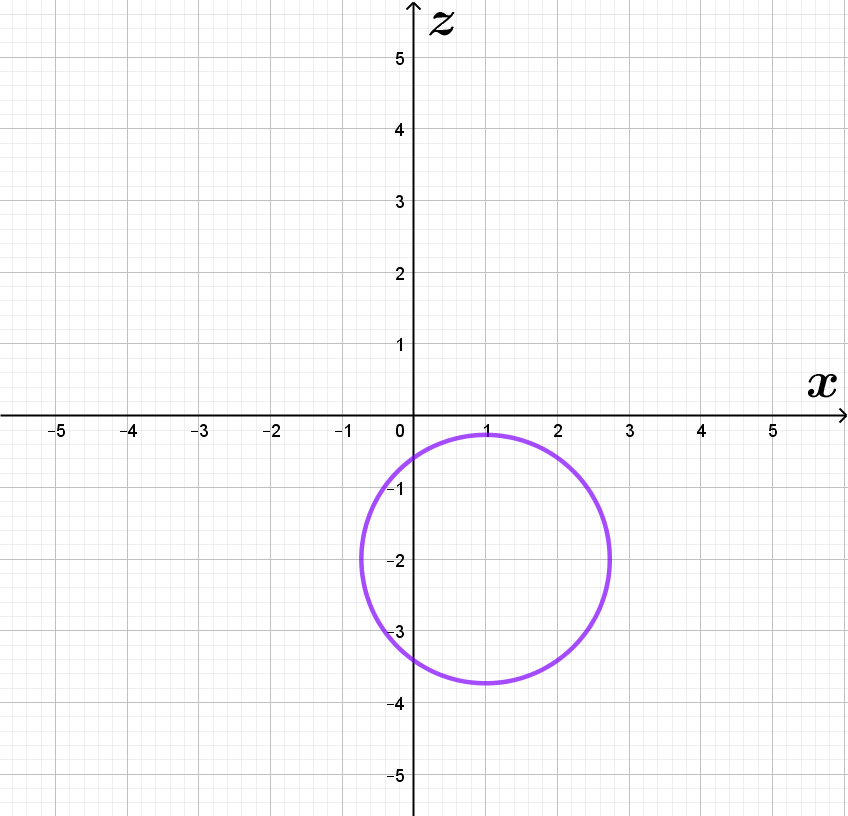
\includegraphics[width=4.5cm]{img/7b2.png}
                        \end{center}
                        En el plano $YZ$:
                        \(
                            x=0 \Rightarrow
                            \frac{1}{2}-\frac{(y-1)^2}{2}+\frac{(z+2)^2}{2}=1\Rightarrow
                            -\frac{(y-1)^2}{2}+\frac{(z+2)^2}{2}=-\frac{1}{2}\Rightarrow
                            (y-1)^2-(z+2)^2=1\Rightarrow
                        \)
                        \begin{center}
                            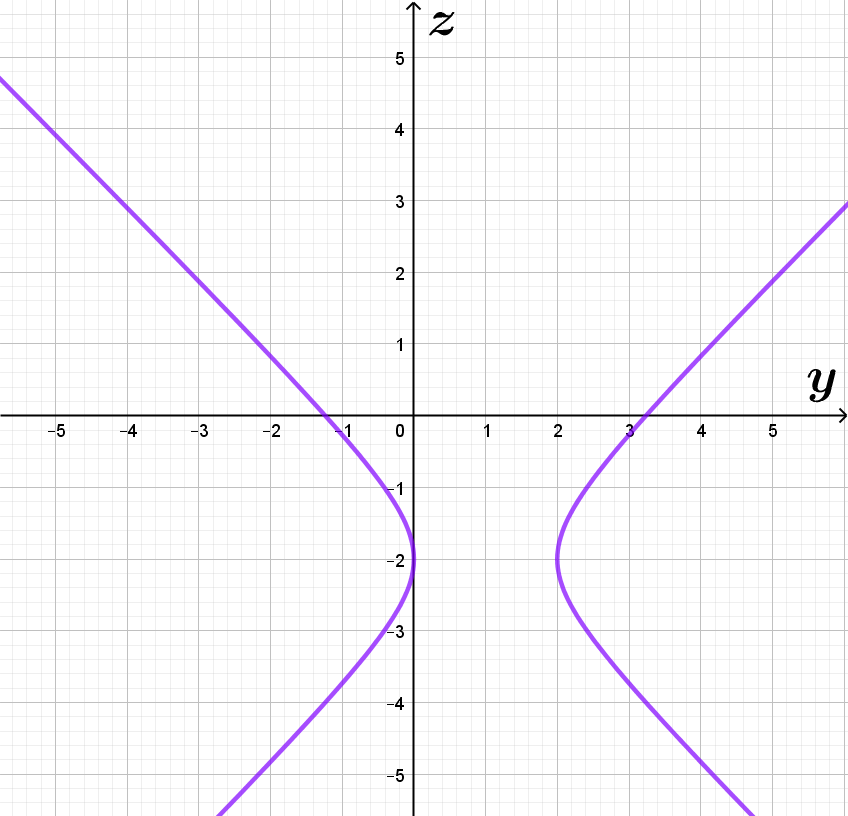
\includegraphics[width=4.5cm]{img/7b3.png}
                        \end{center}
                        La ecuación representa un {\bf hiperboloide de un manto}
                        \begin{center}
                            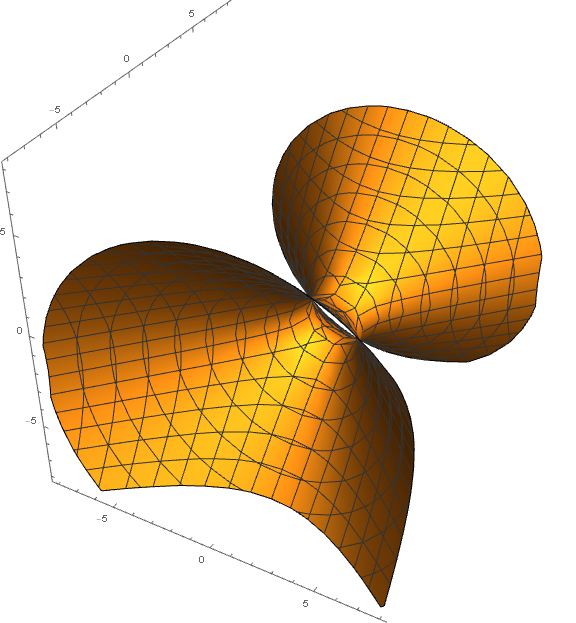
\includegraphics[width=6cm]{img/7b.png}
                        \end{center}
                    }
                \end{enumerate}
            }
        \end{enumerate}
    \end{document}